\documentclass[11pt,xcolor={x11names,svgnames}]{beamer}
\setbeamerfont{note page}{size=\tiny} % default = small 


%\includeonlyframes{applications}


\usecolortheme{rose}
\setbeamertemplate{footline}{}
\setbeamertemplate{navigation symbols}{\footnotesize\insertframenumber}
\usepackage{fontspec}

\setsansfont{PalatinoSansLTPro}[
   Path = /home/charles/charles_work/fonts/PalatinoSans/, 
   Extension      = .otf,
   UprightFont    = *-Regular,
   BoldFont= *-Bold ,
   ItalicFont = *-Italic,
   BoldItalicFont = *-BoldIta
]

\usepackage{graphicx} 
\usepackage{tikz}
\usepackage{xcolor}

\usetikzlibrary{decorations.pathreplacing}
\usetikzlibrary{patterns}

\usepackage{minted}
\usepackage{cellspace}
\usepackage{multirow}
\usetikzlibrary{patterns}
\usetikzlibrary{shapes}

%\usepackage{amssymb, amsmath, amsfonts, amscd}
%\usepackage[noend]{algpseudocode}


\institute[SU] 
{
\vspace*{-0.35cm}
\includegraphics[height=2cm]{pictures/su_logo.png}\hspace{5mm}%
\includegraphics[height=2cm]{pictures/cnrs.jpg}\hspace{5mm}%
\includegraphics[height=2cm]{pictures/LIP6.png}
\vspace*{0.35cm}\\
}

\date{\today}

\title[Seed-Recovery for PCG]{Practical Seed-Recovery for the \\ PCG Pseudo-Random Number Generator}
\author[Bouillaguet, Martinez, Sauvage]{Charles Bouillaguet, Florette Martinez and Julia Sauvage} 

%\includeonlyframes{title,intro,why,pcg,hard_dtl,bragging}


\begin{document}

\begin{frame}[label=title]
  \titlepage
  \begin{tikzpicture}[remember picture,overlay]
    \node<2->[yshift=-1.5cm] at (current page.center) {
      \includegraphics[width=4cm]{charles.jpg}
      \includegraphics[width=4cm]{florette.png}
      \includegraphics[width=4cm]{julia.jpg}
    };
    \node<3->[yshift=-1.5cm,xshift=-0cm,rotate=45,red,scale=4,fill=white,draw,thick,inner sep=1pt] at (current page.center) {\bfseries AWOL};
    \node<3->[yshift=-1.5cm,xshift=4cm,rotate=45,red,scale=4,fill=white,draw,thick,inner sep=1pt] at (current page.center) {\bfseries AWOL};
  \end{tikzpicture}    
\end{frame}


\makeatletter
\newlength\beamerleftmargin
\setlength\beamerleftmargin{\Gm@lmargin}
\makeatother


\section{Introduction}
\begin{frame}<1>[label=intro]
    
    \begin{exampleblock}{What?}
      \begin{itemize}
        
      \item Cryptanalysis of the \textbf{\alert{P}ermuted \alert{C}ongruential \alert{G}enerator}.
      \item Conventional (non-crypto) PRNG
      \end{itemize}
    \end{exampleblock}
    
    \medskip\pause
    
    \begin{alertblock}{Results}
      \textbf{Practical seed-recovery} ($\rightarrow$ prediction) with \textbf{512 output bytes}.
    \end{alertblock}
    
    \begin{block}{How?}
    \begin{itemize}
        \item "Guess-and-Determine" attack.
        \item $\approx 2^{52}$ instances of CVP in dimension 4.
        \item \textbf{Actually done} in $\leq$ 20 000 CPU-hours.
    \end{itemize}  
    \end{block}
\end{frame}

\begin{frame}[label=why]
  \hspace*{-\beamerleftmargin}%
  \includegraphics[width=\paperwidth]{pictures/website.png}
  % \includegraphics[width=12cm]{}
\end{frame}

\begin{frame}[label=why]
    \centering
    \includegraphics[width=\textwidth]{pictures/hard.png}
    \vfill
  \end{frame}

\begin{frame}[label=why]
    \centering
    \includegraphics[width=0.9\linewidth]{pictures/PCG_challenging.jpg}
\end{frame}

\begin{frame}[label=why]
    \centering
    \includegraphics[height=\textheight]{pictures/accepted.jpg}
\end{frame}

\againframe<2>{intro}

\begin{frame}[label=pcg]{Permuted Congruential Generators (\textsf{PCG})}
    \begin{itemize}
    \item Default PRNG in \textsf{NumPy}
      \begin{itemize}
      \item  {\scriptsize ``The fundamental package for scientific computing with Python''}
      \end{itemize}
      
    \item \emph{Filtered} Linear Congruential Generator
    \item ADD vs XOR + (RC5-style) data-dependent rotations
      \medskip
      \begin{itemize}
      \item Internal state : 128-bit
      \item 64-bit outputs
      \item seed : 128-bit initial state +  and 128-bit \alert{increment}
      \end{itemize}
    \end{itemize}

    \begin{center}
    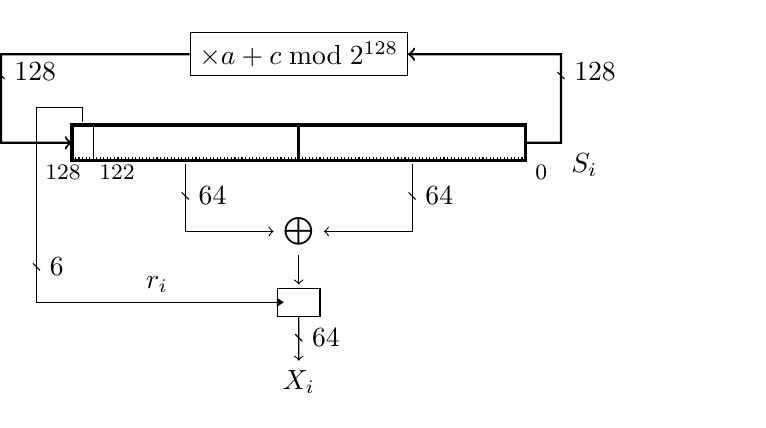
\begin{tikzpicture}[scale=0.45]
      \path[red, use as bounding box] (-1.25, -6.75) rectangle (18.8, 3.75);
      
      % S_i
    
        % bordures
        \draw[very thick]  (0, 0) rectangle (12.8, 1);
        \draw<4->  (0.6, 0) rectangle +(0, 1);
        \draw<3->[very thick]  (6.4, 0) rectangle +(0, 1);
        \foreach \i in {0, 1, ..., 128} \draw (\i/10, 0) -- +(0, 0.1);
        
        % déco autour
        \node<2->[draw] at (6.4, 3) (update) {$\times a + \alert{c} \bmod 2^{128}$};
        \draw<2->[thick,->] (12.8, 0.5) -- (13.8, 0.5) node[below right] {$S_i$} -- (13.8, 3) -- (update);
        \draw<2-> (13.7, 2.5) -- +(0.2, -0.2);
        \path<2-> (13.9, 2.5) node[anchor=west] {128};
        \draw<2->[thick,->] (update) -- (-2, 3) -- (-2, 0.5) node[below left] {$S_{i+1}$} -- (0, 0.5);
        \draw<2-> (-2.1, 2.5) -- +(0.2, -0.2);
        \path<2-> (-1.9, 2.5) node[anchor=west] {128};
    
        
        \node[font=\footnotesize,anchor=west] at (12.8, -0.33) {0};
        %\node<3->[font=\footnotesize,anchor=east] at (6.5, -0.33) {64};
        \node<4->[font=\footnotesize,anchor=west] at (0.5, -0.33) {122};
        \node[font=\footnotesize] at (-0.25, -0.33) {128};
        
        \draw<3-> (6.4, -2) node (x) {$\bigoplus$};
        
        \draw<3->[->] (3.2, -0.1) |- (x);
        \draw<3-> (3.1, -0.9) -- +(0.2, -0.2);
        \path<3-> (3.3, -1) node[anchor=west] {64};
        
        \draw<3->[->] (9.6, -0.1) |- (x);
        \draw<3-> (9.5, -0.9) -- +(0.2, -0.2);
        \path<3-> (9.7, -1) node[anchor=west] {64};
    
        \node<4>[minimum width=1.8cm] at (6.4, -4) (r) {$\ggg$};
        \draw<4> (5.8, -3.6) rectangle +(1.2, -0.8);
        \draw<4>[fill=black] (5.8, -4.1) -- (5.95, -4) -- (5.8, -3.9) -- cycle;
        
        \draw<4> (0.3, 1.1) -- (0.3, 1.5) -- (-1, 1.5) -- (-1, -4) -- node[above] {$r_i$} (5.8, -4);
        \draw<4> (-1.1, -2.9) -- +(0.2, -0.2);
        \path<4> (-0.9, -3) node[anchor=west] {6};
    
        \draw<3->[->] (x) -- +(0, -1.5);
        \node<4> at (6.4, -6.25) (xi) {$X_i$};
        \draw<4>[->] (6.4, -4.4) -- (xi);
    
        \draw<4> (6.3, -4.9) -- +(0.2, -0.2);
        \path<4> (6.5, -5) node[anchor=west] {64};
      \end{tikzpicture}
    \end{center}

  \end{frame}



%%%%%%%%%%%%%%%%%%%%%%%


\begin{frame}[label=hard_dtl]{The Attack}

\begin{figure}
\begin{center}
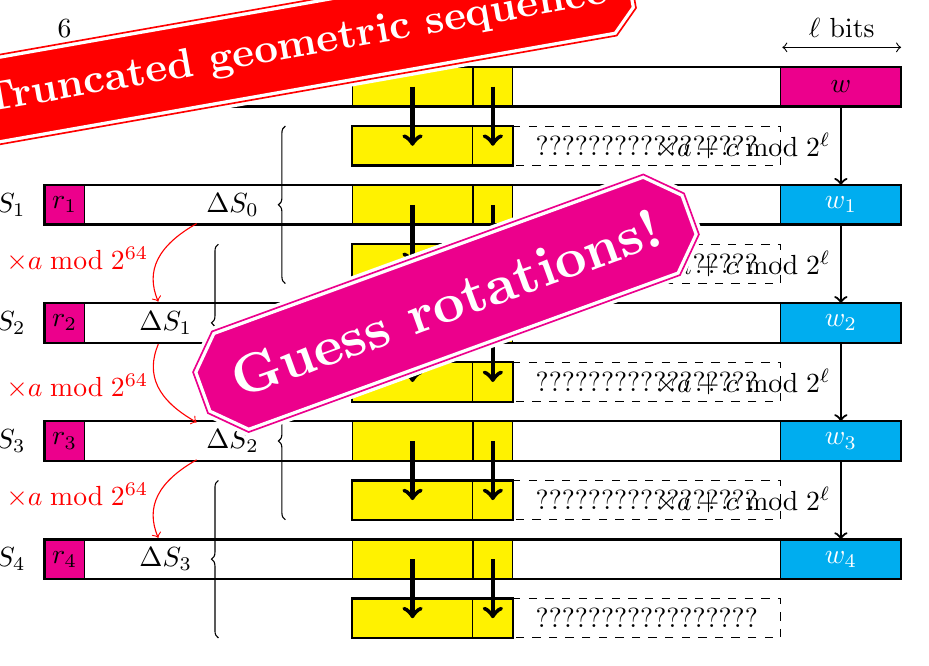
\begin{tikzpicture}[xscale=0.85, yscale=0.5]
  \path[red, use as bounding box] (-0.25, -13.5) rectangle (12.8, 2);
  
  % S_0
  \begin{scope}
    % remplissage
    \fill<4-5>[fill=yellow] (4.6, 0) rectangle +(2.4, 1);
    \fill<2-5>[fill=magenta] (0, 0) rectangle node {$r_0$} +(0.6, 1);
    \fill<2-5>[fill=magenta] (11, 0) rectangle node {$w$} +(1.8, 1);
    
    % bordures
    \draw<1-5>[thick]  (0, 0) rectangle (12.8, 1);
    \draw<2-5>  (0.6, 0) rectangle +(0, 1);
    \draw<1-5>[thick]  (6.4, 0) rectangle +(0, 1);
    \draw<4-5>  (7.0, 0) rectangle +(0, 1);
    \draw<4-5> (4.6, 0) rectangle +(0, 1);
    \draw<2-5>  (11, 0) rectangle +(0, 1);
    
    % déco autour
    \node<1-5> at (-0.5, 0.5) {$S_0$};
    \draw<2-5>[<->] (12.8, 1.5) -- node[above] {$\ell$ bits} +(-1.775, 0);
    \draw<2-5>[<->] (0, 1.5) -- node[above] {6} +(0.6, 0);
  \end{scope}

  % T_0
  \begin{scope}[xshift=4.6cm, yshift=-1.5cm]    
    \draw<5->[dashed]  (0, 0) rectangle +(6.4, 1);
    \draw<5->[thick,fill=yellow]   (0, 0) rectangle +(2.4, 1);
    \draw<5>[]   (1.8, 0) rectangle +(0, 1);
    \path<5->  (2.4, 0) rectangle node {$?????????????????$} (6.4, 1);
  \end{scope}

  % flèches S_i --> T_i
  \draw<5> [ultra thick,->] (5.5, 0.5) -- +(0, -1.5);
  \draw<5> [ultra thick,->] (6.7, 0.5) -- +(0, -1.5);

  
  %%%%%%%%%

  
  % S_1
  \begin{scope}[yshift=-3cm]
    % remplissage
    \fill<4-5>[fill=yellow] (4.6, 0) rectangle +(2.4, 1);
    \fill<2-5>[fill=magenta] (0, 0) rectangle node {$r_1$} +(0.6, 1);
    \fill<3-5>[fill=cyan] (11, 0) rectangle node[text=white] {$w_1$} +(1.8, 1);
    
    % bordures
    \draw<1-5>[thick]  (0, 0) rectangle (12.8, 1);
    \draw<2-5>  (0.6, 0) rectangle +(0, 1);
    \draw<1-5>[thick]  (6.4, 0) rectangle +(0, 1);
    \draw<4-5>  (7.0, 0) rectangle +(0, 1);
    \draw<4-5>  (4.6, 0) rectangle +(0, 1);
    \draw<3-5>  (11, 0) rectangle +(0, 1);
    
    % déco autour
    \node<1-5> at (-0.5, 0.5) {$S_1$};
  \end{scope}
  
  % T_1
  \begin{scope}[xshift=4.6cm, yshift=-4.5cm]    
    \draw<5->[dashed]  (0, 0) rectangle +(6.4, 1);
    \draw<5->[thick,fill=yellow]  (0, 0) rectangle +(2.4, 1);
    \draw<5>[]  (1.8, 0) rectangle +(0, 1);
    \path<5-> (2.4, 0) rectangle node {$?????????????????$} (6.4, 1);
  \end{scope}

  \begin{scope}[yshift=-3cm]
    % flèches S_i --> T_i
    \draw<5>[ultra thick,->] (5.5, 0.5) -- +(0, -1.5);
    \draw<5>[ultra thick,->] (6.7, 0.5) -- +(0, -1.5);
  \end{scope}

  
  %%%%%%%%%%%%%

  
  % S_2
  \begin{scope}[yshift=-6cm]
    % remplissage
    \fill<4-5>[fill=yellow] (4.6, 0) rectangle +(2.4, 1);
    \fill<2-5>[fill=magenta] (0, 0) rectangle node {$r_2$} +(0.6, 1);
    \fill<3-5>[fill=cyan] (11, 0) rectangle node[text=white] {$w_2$} +(1.8, 1);
    
    % bordures
    \draw<1-5>[thick]  (0, 0) rectangle (12.8, 1);
    \draw<2-5>  (0.6, 0) rectangle +(0, 1);
    \draw<1-5>[thick]  (6.4, 0) rectangle +(0, 1);
    \draw<4-5>  (7.0, 0) rectangle +(0, 1);
    \draw<4-5>  (4.6, 0) rectangle +(0, 1);
    \draw<3-5>  (11, 0) rectangle +(0, 1);
    
    % déco autour
    \node<1-5> at (-0.5, 0.5) {$S_2$};
  \end{scope}    
  
  % T_2
  \begin{scope}[xshift=4.6cm, yshift=-7.5cm]    
    \draw<5->[dashed]  (0, 0) rectangle +(6.4, 1);
    \draw<5->[thick,fill=yellow]  (0, 0) rectangle +(2.4, 1);
    \draw<5>[]  (1.8, 0) rectangle +(0, 1);
    \path<5-> (2.4, 0) rectangle node {$?????????????????$} (6.4, 1);
  \end{scope}

  \begin{scope}[yshift=-6cm]
    % flèches S_i --> T_i
    \draw<5>[ultra thick,->] (5.5, 0.5) -- +(0, -1.5);
    \draw<5>[ultra thick,->] (6.7, 0.5) -- +(0, -1.5);
  \end{scope}

  
  %%%%%%%%%%%%%

  
  % S_3
  \begin{scope}[yshift=-9cm]
    % remplissage
    \fill<4-5>[fill=yellow] (4.6, 0) rectangle +(2.4, 1);
    \fill<2-5>[fill=magenta] (0, 0) rectangle node {$r_3$} +(0.6, 1);
    \fill<3-5>[fill=cyan] (11, 0) rectangle node[text=white] {$w_3$} +(1.8, 1);
    
    % bordures
    \draw<1-5>[thick]  (0, 0) rectangle (12.8, 1);
    \draw<2-5>  (0.6, 0) rectangle +(0, 1);
    \draw<1-5>[thick]  (6.4, 0) rectangle +(0, 1);
    \draw<4-5>  (7.0, 0) rectangle +(0, 1);
    \draw<4-5>  (4.6, 0) rectangle +(0, 1);
    \draw<3-5>  (11, 0) rectangle +(0, 1);
    
    % déco autour
    \node<1-5> at (-0.5, 0.5) {$S_3$};
   \end{scope}

  % T_3
  \begin{scope}[xshift=4.6cm, yshift=-10.5cm]    
    \draw<5->[dashed]  (0, 0) rectangle +(6.4, 1);
    \draw<5->[thick,fill=yellow]  (0, 0) rectangle +(2.4, 1);
    \draw<5>[]  (1.8, 0) rectangle +(0, 1);
    \path<5-> (2.4, 0) rectangle node {$?????????????????$} (6.4, 1);
  \end{scope}

  \begin{scope}[yshift=-9cm]
  % flèches S_i --> T_i
    \draw<5>[ultra thick,->] (5.5, 0.5) -- +(0, -1.5);
    \draw<5>[ultra thick,->] (6.7, 0.5) -- +(0, -1.5);
  \end{scope}
  
    %%%%%%%%%%%%%

  
  % S_4
  \begin{scope}[yshift=-12cm]
    % remplissage
    \fill<4-5>[fill=yellow] (4.6, 0) rectangle +(2.4, 1);
    \fill<2-5>[fill=magenta] (0, 0) rectangle node {$r_4$} +(0.6, 1);
    \fill<3-5>[fill=cyan] (11, 0) rectangle node[text=white] {$w_4$} +(1.8, 1);
    
    % bordures
    \draw<1-5>[thick]  (0, 0) rectangle (12.8, 1);
    \draw<2-5>  (0.6, 0) rectangle +(0, 1);
    \draw<1-5>[thick]  (6.4, 0) rectangle +(0, 1);
    \draw<4-5>  (7.0, 0) rectangle +(0, 1);
    \draw<4-5>  (4.6, 0) rectangle +(0, 1);
    \draw<3-5>  (11, 0) rectangle +(0, 1);
    
    % déco autour
    \node<1-5> at (-0.5, 0.5) {$S_4$};
  \end{scope}    

  % T_4
  \begin{scope}[xshift=4.6cm, yshift=-13.5cm]    
    \draw<5->[dashed]  (0, 0) rectangle +(6.4, 1);
    \draw<5->[thick,fill=yellow]  (0, 0) rectangle +(2.4, 1);
    \draw<5>[]  (1.8, 0) rectangle +(0, 1);
    \path<5-> (2.4, 0) rectangle node {$?????????????????$} (6.4, 1);
  \end{scope}
  \begin{scope}[yshift=-12cm]
  % flèches S_i --> T_i
    \draw<5>[ultra thick,->] (5.5, 0.5) -- +(0, -1.5);
    \draw<5>[ultra thick,->] (6.7, 0.5) -- +(0, -1.5);
  \end{scope}

  
  % Differences
  \begin{scope}[xshift=4.6cm, decoration={brace,mirror},>=stealth]  
    \draw<6->[decorate]  (-1, -0.5) -- +(0, -4);
    \node<6->[anchor=east] at (-1.25, -2.5)  (T0) {$\Delta S_0$};
  \end{scope}

  % Differences
  \begin{scope}[xshift=3.6cm, yshift=-3cm, decoration={brace,mirror},>=stealth]  
    \draw<6->[decorate]  (-1, -0.5) -- +(0, -4);
    \node<6->[anchor=east] at (-1.25, -2.5)  (T1) {$\Delta S_1$};
  \end{scope}

  % Differences
  \begin{scope}[xshift=4.6cm, yshift=-6cm, decoration={brace,mirror},>=stealth]  
    \draw<6->[decorate]  (-1, -0.5) -- +(0, -4);
    \node<6->[anchor=east] at (-1.25, -2.5)  (T2) {$\Delta S_2$};
  \end{scope}

  % Differences
  \begin{scope}[xshift=3.6cm, yshift=-9cm, decoration={brace,mirror},>=stealth]  
    \draw<6->[decorate]  (-1, -0.5) -- +(0, -4);
    \node<6->[anchor=east] at (-1.25, -2.5)  (T3) {$\Delta S_3$};
  \end{scope}

  % arrows
  \draw<7->[red,->] (T0) edge[bend right] node[left] {$\times a \bmod 2^{64}$} (T1);
  \draw<7->[red,->] (T1) edge[bend right] node[left] {$\times a \bmod 2^{64}$} (T2);
  \draw<7->[red,->] (T2) edge[bend right] node[left] {$\times a \bmod 2^{64}$} (T3);

  % flèches w
  \draw<3>[thick,->] (11.9, 0) -- node[left] {$\times a + c \bmod \alert{2^\ell}$} +(0, -2);
  \draw<3>[thick,->] (11.9, -3) -- node[left] {$\times a + c \bmod \alert{2^\ell}$} +(0, -2);
  \draw<3>[thick,->] (11.9, -6) -- node[left] {$\times a + c \bmod \alert{2^\ell}$} +(0, -2);
  \draw<3>[thick,->] (11.9, -9) -- node[left] {$\times a + c \bmod \alert{2^\ell}$} +(0, -2);
  

    \node<2>[scale=2,rotate=20,chamfered rectangle, white, fill=magenta, double=magenta, draw, very thick] at (6, -5) {\bfseries Guess rotations!};

  
  \node<7>[scale=1.5,rotate=10,chamfered rectangle, white, fill=red, double=red, draw, very thick] at (3.75, 1.5) {\bfseries Truncated geometric sequence};
\end{tikzpicture}
\end{center}
\end{figure}
\end{frame}

%%%%%%%%%%%%%%%%%%%%%%%%%%%%%%%%%%%%%%%%%%%%%%%%%%%%%%%%%%%%

\begin{frame}[label=lattice]
\hspace*{-\beamerleftmargin}%
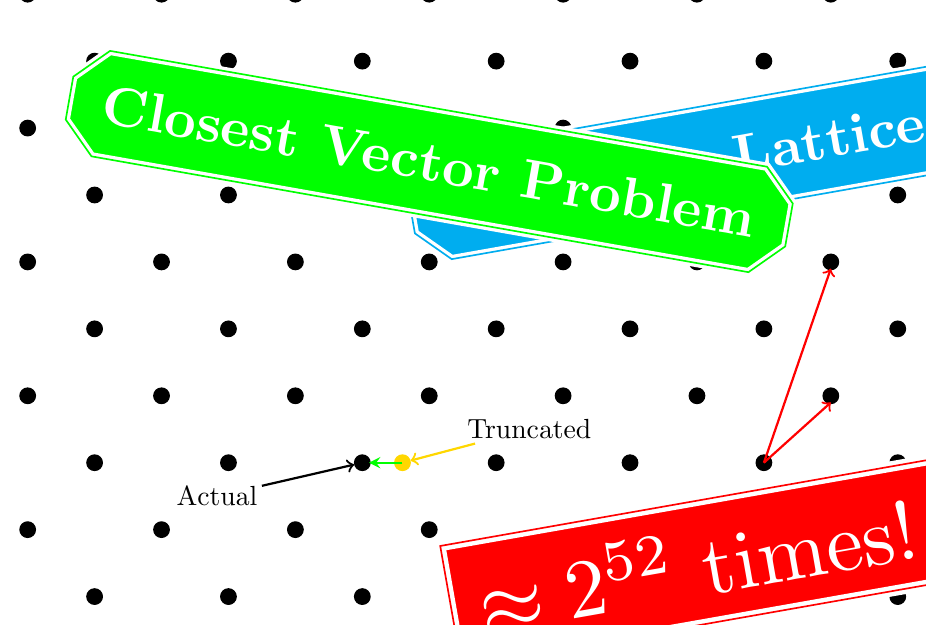
\begin{tikzpicture}[scale=0.85]
    \path[use as bounding box] (-5, -2) rectangle (8, 6.5);
    \foreach \x in {-3,-2,-1,0,1,2,3,4,5}{
		\foreach \y in {-2,-1,0,1,2,3}{
			\node[draw,circle,inner sep=2pt,fill] at (2*\x,2*\y) {};
			\node[draw,circle,inner sep=2pt,fill] at (2*\x+1,2*\y+1) {};
			
		}
	}
    \draw[->,thick,red] (6,0) --(7,2.9);
    \draw[->,thick,red] (6,0) --(7,0.9);
    
    \node<2->[draw,circle,inner sep=2pt,Gold,fill] at (2*0.3, 0) (trunc) {};
    \node<2->[anchor=west,inner sep=1.5pt] at (1.5, 0.5) (trunc_label) {Truncated};
    \draw<2->[Gold, thick, ->] (trunc_label) edge (trunc);

    \node[shape=circle,inner sep=2pt] at (0, 0) (rec) {};
    \node<2->[anchor=east,inner sep=1.5pt] at (-1.5, -0.5) (rec_label) {Actual};
    \draw<2->[thick, ->] (rec_label) edge (rec);

    
    \draw<3->[draw,thick,green,->,>=stealth] (2*0.3, 0) -- +(-0.5, 0);

    \node<1>[scale=2,rotate=10,chamfered rectangle, white, fill=cyan, double=cyan, draw, very thick] at (5, 4.5) {\bfseries Euclidean Lattices};


    \node<4->[scale=2,rotate=-10,chamfered rectangle, white, fill=green, double=green, draw, very thick] at (1, 4.5) {\bfseries Closest Vector Problem};

    \node<5>[scale=3,rotate=10, rectangle, white, fill=red, double=red, draw, ultra thick] at (5, -1.5) {$\approx 2^{52}$ times!};

    
\end{tikzpicture}
\end{frame}



%%%%%%%%%%%%%%%%%%%%%%%%%%%%%%%%%%%%%%%%%%%%%%%%%%%%%%%%%%%%%%%%%

\begin{frame}[label=bragging]
  \begin{columns}
    \begin{column}[T]{3.5cm}
      \includegraphics[height=0.6\textheight]{pictures/jean-zay.jpg}
    \end{column}
    \begin{column}[T]{6cm}
      \includegraphics[width=\textwidth]{pictures/jean_Zay.jpg}

      \begin{itemize}
      \item Implementation effort...
      \item ... + Big Iron
        \medskip
      \item Requested stream from designer, emailed back seed

      \end{itemize}
    \end{column}
  \end{columns}

  \medskip
  
  \begin{itemize}
  \item Running time: \textbf{35 minutes} {\tiny (using 20480 cores)}
    \medskip
    \begin{itemize}\footnotesize
    \item 1024 $\times$ 20-core \textsf{Xeon Gold 6248 @ 2.5Ghz}
    \end{itemize}
  \end{itemize}
  \end{frame}

%%%%%%%%%%%%%%%%%%%%%%%%%%%

  \begin{frame}

    \begin{exampleblock}{Details ?}
      \begin{center}
      
\begin{tikzpicture}
        \node[scale=2,rotate=6, chamfered rectangle, white, fill=red, double=red, draw, ultra thick] at (0,0) {Go read the full paper!};
      \end{tikzpicture}
    \end{center}
  \end{exampleblock}

    \bigskip

\begin{block}{Take-Home Message}
  \begin{itemize}
    \item Reconstructing the seed for PCG is \textbf{practical}.
    \item PCG is \textbf{not} cryptographically secure (never claimed to be).
    \item \textbf{Don't} use \textsf{Numpy} to generate nonces...
    \end{itemize}
  \end{block}
\end{frame}


\end{document}


%%% Local Variables:
%%% TeX-command-extra-options: "-shell-escape"
%%% ispell-local-dictionary: "english"
%%% TeX-engine: xetex
%%% eval: (flyspell-mode 1)
%%% eval: (reftex-mode 1)
%%% End:
